\documentclass[a4paper,12pt]{article}
   % Packages and definitions:
   % {
      \usepackage{float}
      \usepackage[english]{babel}
      \usepackage[utf8]{inputenc}
      \usepackage{amsmath}
      \usepackage{amssymb}
      \usepackage{color}
      \usepackage{subcaption}
      \usepackage{booktabs}
      \usepackage{tikz}
      \usepackage{multirow}
      \usetikzlibrary{decorations.pathreplacing}
      \usepackage{graphicx,epstopdf}
      \usepackage{cleveref}
      \usepackage{collcell} % loads array
      \usepackage{listings}
      \usepackage{algorithm}
      \usepackage{siunitx}
      \usepackage{algpseudocode}
      \newcolumntype{m}{>{$} r <{$}}
      \newcolumntype{u}{>{$[\collectcell\si} l <{\endcollectcell]$}}
      \newcommand{\approxtext}[1]{\ensuremath{\stackrel{\text{#1}}{=}}}
      \newcommand{\matr}[1]{\mathbf{#1}}
      \newcommand{\partt}[2]{\ensuremath{\dfrac{\d {#1}}{\partial {#2}}}}
      \renewcommand{\d}[1]{\ensuremath{\operatorname{d}\!{#1}}} % non-italized differentials
      \newcommand{\h}[0]{\ensuremath{\hbar}} % hbar
      \newcommand{\qed}[0]{\ensuremath{\tag*{$\square$}}} % QED square
      \def\changemargin#1#2{\list{}{\rightmargin#2\leftmargin#1}\item[]}
      \let\endchangemargin=\endlist 
      \usepackage{amsthm}
      \theoremstyle{plain}
      \newtheorem{thm}{theorem} % reset theorem numbering for each chapter
      \theoremstyle{definition}
      \newtheorem{defn}[thm]{definition} % definition numbers are dependent on theorem numbers
      \newtheorem{exmp}[thm]{example} % same for example numbers
      \bibliographystyle{natbib}
      \renewcommand{\theequation}{\thesection.\arabic{equation}}
      \newcommand{\ts}{\textsuperscript} 

      \definecolor{dkgreen}{rgb}{0,0.6,0}
      \definecolor{gray}{rgb}{0.5,0.5,0.5}
      \definecolor{mauve}{rgb}{0.58,0,0.82}

      \lstset{frame=tb,
        language=Java,
        aboveskip=3mm,
        belowskip=3mm,
        showstringspaces=false,
        columns=flexible,
        basicstyle={\small\ttfamily},
        numbers=none,
        numberstyle=\tiny\color{gray},
        keywordstyle=\color{blue},
        commentstyle=\color{dkgreen},
        stringstyle=\color{mauve},
        breaklines=true,
        breakatwhitespace=true,
        tabsize=3
      }
% }
\title
{
	\textbf
	{
      How hot is my hot chocolate? \\Partial differential equations for an ideal
      thermos
   }
}

\author{Henrik Åhl\\
\small{in collaboration with Denhanh Huynh}}
\date{\today}

\begin{document}
\begin{titlepage}
	
   \maketitle 
	\begin{center}
		\phantom{a}
		{Department of Astronomy and Theoretical Physics, Lund University}
		\\[2cm]
		{Project supervised by Tobias Ambjörnsson}
		\vfill
		\includegraphics[height=4cm]{logocLUeng.pdf}
	\end{center}
	\thispagestyle{empty} % do not count pages just yet

\end{titlepage}

\section{Introduction}
   Partial differential equations link the simultaneous changes in several
   variables to the ultimate change in the corresponding function itself. The
   amount of applications are of course numerous, but in particular partial
   differential equations, or henceforth \emph{PDE's}, can be used to describe
   the change in heat throughout liquids, gases and solids. The so called
   \emph{heat equation} links all these together through the identity
      \begin{align*}
         \frac{\partial T}{\partial t} - \nabla^2 u = 0
      \end{align*}
   where $T = T(\mathbf r,t)$. In this report we will limit ourselves to the
   one-dimensional case, so that $\mathbf r = x\hat x$, and focus on the
   numerical calculation of how the heat spreads in an open, ideal thermos. 

\section{Solving the heat equation numerically}
	\setcounter{equation}{0}
   \subsection{Description of the problem}
      Jonathan is out on a warm winter day skiing, having brought his new
      futuristic super-thermos \emph{ThermaHold\texttrademark}\hspace{2pt}\footnote{Patent
      pending.} with him. Imsy-wimsy Jonathan however, off onto new adventures, 
      manages to forget his thermos left open in the snow. How long will it take before 
      Jonathan's thermos full of hot chocolate has turned cold? What if Jonathan
      has added his daily nutrient pill to the hot beverage, effectively raising
      the diffusivity? What if the whole pill does not dissolve completely? 

      The explicit euler method is used for calculating the increment due to
      steps in time. This method is chosen because of the simplicity and the
      merits with respect to the computation time. No matrix inversions are for
      example needed, as tends to be the case in the Crank-Nicholson method. The
      explicit euler method is however of second order in space and first order
      in time, whereas the Crank-Nicholson algorithm renders a result that is on
      par in space and in second order in time (due to using the second
      derivative to approximate the function). However, the lack of matrix operations
      required for the explicit euler case outweighs the benefits of a more
      accurate algorithm. The same argument applies for the implicit euler
      method, as a matrix inversion is required in that case. In short: a more
      complicated model is simply not needed for our problem. The greatest limitation 
      of the explicit method is simply mainly the restriction in the
      relation between the time and space step -- a hindrance the implicit
      methods both avoid. 
      
   
   \subsection{A numerical approximation}
      Knowing from pre-university mathematics, the first derivative of a
      function can be roughly approximated by the slope between two points along
      the curve. For a function $T$ that is, it means that the first derivate
      at a point $j$ would approximately equal, through the forward difference
      method, 
         \begin{align}
            \frac{\partial T_{j}}{\partial x} \approx \frac{T_{j+1} - T_j}{a}
            \label{eq:first_der}
         \end{align}
      for some step size $a$, when the dimension $\hat x$ is discretized so that
      $x_j = ja$. This can be done recursively, since the same reasoning applies
      to the second derivative, so that it resultingly can be written as
         \begin{align}
            \frac{\partial^2 T_{j}}{\partial x^2} \approx \frac{T_{j+1} - 2T_j + T_{j-1}}{a^2},
            \label{eq:second_der}
         \end{align}
      here instead using the backward difference.
   
      This all implies that the diffusion equation can be written as a system of
      first-order ordinary differential equations, such that 

      \begin{align}
         \matr A = \frac{D}{a^2} 
         \left(
         \begin{matrix}
            &&&&& \\
            \ddots & \ddots & \ddots &        & 0      & \\
                   & 1      & -2     & 1      &        & \\
                   &        & 1      & -2     & 1      & \\
                   & 0      &        & \ddots & \ddots & \ddots \\
            &&&&& 
             \end{matrix} \right)
         \label{eq:matrix}
      \end{align}

      Discretizing with respect to time as well, i.e. stating that $t_n = nh$
      for some constant step size in time $h$, one can solve the resulting
      equation using the \emph{explicit euler method} through realizing that
      
      \begin{align}
         \frac{\mathbf T^{n+1} - \mathbf T^n}{h} = \matr A \mathbf T^n
         \label{eq:explicit_euler}
      \end{align}
      for all $\mathbf T^n$ such that $\mathbf T^n = \mathbf T(t_n)$. 
      This method is stable for all solutions as long as $h \leq a^2/2$.  
     
      Because of the one-sided boundary conditions (see \cref{sec:bc}), the last
      value was calculated via a backward step instead of a forward one, so as
      to limit the value at the bottom. Correspondingly, the first value of
      $\mathbf u$ was set to correspond to the direct outerward boundary condition.
      From a practical perspective, this allows for direct computation of the
      vector $\mathbf u^{n+1}$ via matrix multiplication.

      The computation speed for the system ought furthermore scale quadratically
      with time due to the quadric nature of the matrix $\matr A$. 

   \subsection{Simulation settings and boundary conditions}
      \label{sec:bc}
      The simulations were performed assuming that the thermos is completely
      isolated due to the high tecnological capabilities of a
      \emph{ThermaHold\texttrademark}, aside from the open top. The simulations
      use the diffusivity constant for water at $T=25^\circ$C, $D = 0.14 \cdot
      10^{-6}~\si{\meter^2\per\s}$~\cite{diffusion}, and
      boundary temperatures 
      \begin{align*}
         T(x = 0,t)  &=  0~^\circ\text{C} \\
         T(x, t = 0) &=  90~^\circ\text{C} \\
      \end{align*}
      as well as step sizes $a = 1.0\cdot 10^{-3}~\si{\m}$ and $h \lesssim 5.0\cdot
      10^{-6}~\si{\m}$. The size of the thermos is set to 0.30 m.      

\section{Results and conclusions}
   The results prove that indeed, the temperature spread throughout the depth of
   the thermos is apparent. Due to the extremely high functionality however,
   which is to say the very ideal conditions, the case based on the realistic
   heat diffusivity constant $D$ is extremely slowly developing, resulting in a
   final mean temperature of roughly the initial one, as can be seen in
   \cref{fig:mean}. The reader should here note that time is given in the numbers
   of hours passed since the start of the simulation, whereas the position value
   corresponds to the relevant cell (due to the discretization).
   
   \Cref{fig:normal} shows, however, the intended dynamics of
   the model, which is that the surface-aligned cell will decrease in
   temperature the fastest, bringing on a slower, but steady development for the
   after-coming cells. 
   
   Notably, the spread over time towards the cells lying deeper inside the
   thermos is visible in \cref{fig:normal}, as the slope in the $x$--$y$ plane
   is evident. The effect is even clearer when the diffusion constant is changed
   somewhat, to
   a value on the order $10^-1$, as is visualized in~\cref{fig:new}.

   \begin{figure}[H]
      \centering
      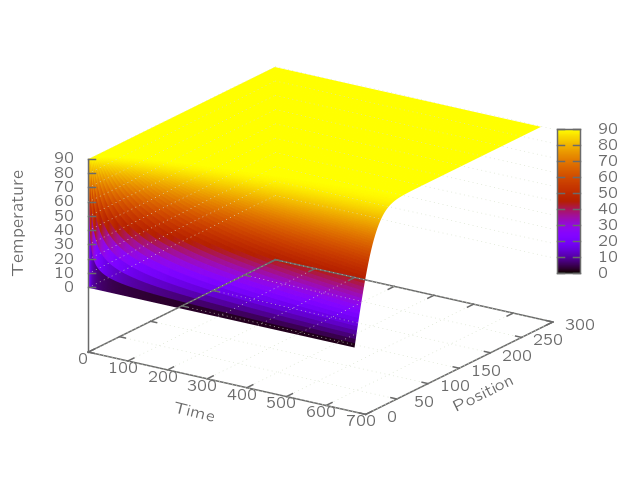
\includegraphics[width=0.8\textwidth]{../script/testout.png}
      \caption{Temperature development with respect to space and time. Positions
      are given in the cell number inherent to the discretization, i.e. in this
      case the step parameter $j$.}
      \label{fig:normal}
   \end{figure}       
   \begin{figure}[H]
      \centering
      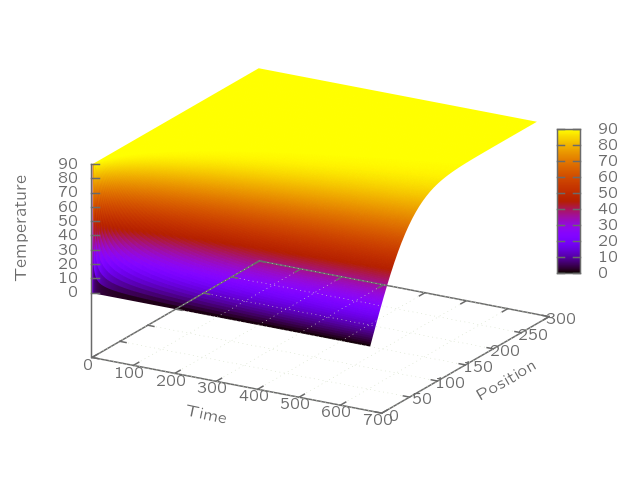
\includegraphics[width=0.8\textwidth]{../test.png}
      \caption{Temperature development with respect to space and time. Positions
      are given in the cell number inherent to the discretization, i.e. in this
      case the step parameter $j$.}
      \label{fig:new}
   \end{figure}       
   
   When the model is adjusted so that the diffusitivity constant is increased by
   a value on the order of $10^6$ times the original value, the mean
   temperature in the thermos decreases significantly more rapidly, although it
   still takes about four full days for the mean temperature to rougly reach the
   outside temperature. Although this implies issues with our model, it
   signifies the affectance the ideal conditions have on the outcome. The
   temperature development on the other hand, as can be seen in \cref{fig:01},
   shows a much stronger bias towards time than towards position over the course
   of the first days, which does not conflict with the expectations for the
   outcome markedly.


   \begin{figure}[H]
      \centering
      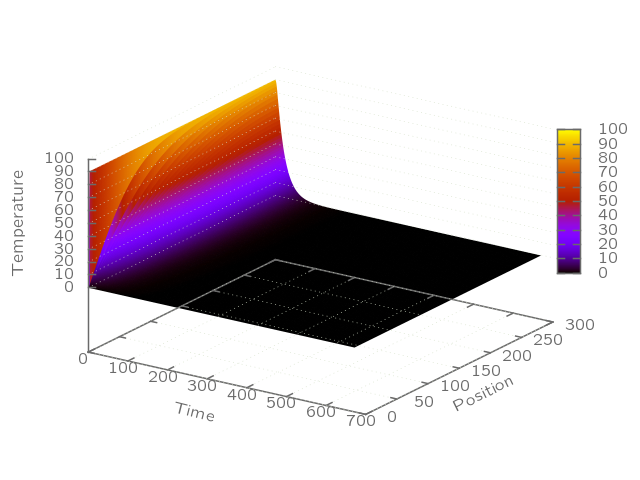
\includegraphics[width=0.8\textwidth]{../script/01fig.png}
      \caption{Temperature development with the heat diffusivity raising pill
      added to the mixture. Compare with the mean temperate over time in
   \cref{fig:mean}.}
      \label{fig:01}
   \end{figure}       
   \begin{figure}[H]
      \centering
      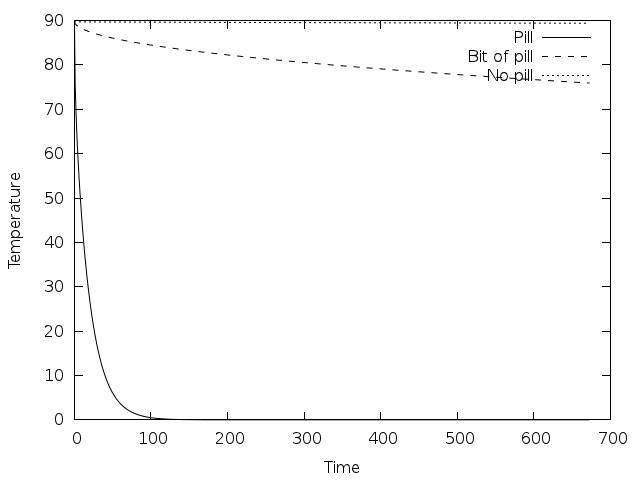
\includegraphics[width=0.8\textwidth]{../script/all.png}
      \caption{Mean temperature over the course of a total of four weeks. Note
      that the ``Pill'' labels signify different diffusion constants from the
      original one.}
      \label{fig:mean}
   \end{figure}       

   In conclusion, our model has showed the significant impacts idealization can
   have on the outcome of simulations. The results do not provide realistical
   data, but can be of interest to understand the dynamics of heat diffusion in
   a near-ideal case. 

\newpage

\begin{thebibliography}{99}
   \bibitem{lecnotes}
      Tobias Ambjörnsson,
     \emph{Lecture notes, Computational Physics},
     Department of Astronomy and Theoretical Physics,
     Lund University,
     2015.
 
   \bibitem{diffusion}
      J. Blumm, A. Lindemann,
      \emph{Characterization of the thermophysical properties of molten polymers
      and liquids using the flash technique},
      High Temperatures -- High Pressures 35/36 (6)
      2007.

\end{thebibliography}
\newpage
\appendix
\section{Code}
   \label{sec:code}
   \lstinputlisting[language=Java]{/home/henrik/gitter/pde/pde/src/pde/Thermos.java}
\end{document}

